\section{强子衰变模拟}
\label{ch:cocktail}
在本分析当中测量双电子谱时并没有对物理过程进行具体的挑选,最后所得到的双电子谱是多个物理过程的双电子谱叠加所的到的谱。此分析当中我们感兴趣的物理过程是$\rho$介子的质量谱和直接来自于夸克胶子等离子体热辐射的双电子谱。相对于这两个过程而言,来源于其他过程的双电子谱在本分析当中被我们视为背景过程。为了能从总的双电子谱中抽取来自于感兴趣的物理过程的双电子谱,在本分析中所用到的方法是通过模拟的方法得到来自于背景过程的双电子谱,再将这些来自于背景过程双电子模拟谱从测量得到的双电子谱中扣除。所剩的即为感兴趣的物理过程的双电子谱。这个对背景过程的模拟就是强子衰变模拟。因为所需模拟的过程很多并且最后会加在一起,就像调制鸡尾酒一般,所以又叫做hadronic cocktail。

背景过程主要有有以下几种:
\begin{itemize}
    \item 强子两体衰变,如$\omega \rightarrow e^+e^-$,$\phi \rightarrow e^+e^-$,$J/\psi \rightarrow e^+e^-$。
    \item 强子三体衰变(Dalitz decay),如$\pi^0 \rightarrow \gamma e^+e^-$,$\eta \rightarrow \gamma e^+e^-$,$\eta^\prime \rightarrow \gamma e^+e^-$,$\omega \rightarrow \gamma e^+e^-$,$\phi \rightarrow \gamma e^+e^-$
    \item 重味夸克半轻子衰变,如$c\bar{c} \rightarrow e^+e^-+X$
    \item Drell-Yan过程
\end{itemize}
在接下来的几个小节里面会对这些不同的过程的模拟方式进行具体的讨论。

\subsection{强子两体及三体衰变}

首先是从强子两体或三体衰变得到的双电子谱,其中衰变过程包括两体衰变和三体衰变两种过程。这两种过程的主要区别在于母粒子的质量分布有所不同。下文中会进行具体讨论。在模拟过程中,首先要确定母粒子的各个动力学相关项的分布。其中包括母粒子的方位角、快度、横动量和质量分布,在下文当中会对这些分布进行具体地讨论。

母粒子的方位角分布和计算电子对探测效率时的虚光子模拟相同,这些母粒子的方位角分布也是各向同性的,为在$-\pi~-~\pi$区间内均匀分布。

对于快度的分布,在STAR之前200 GeV金-金对撞和193 GeV铀-铀对撞的双电子分析当中采用的是 -1 - 1范围内的均匀分布。在较低对撞质心能量的情况下,为了更好地描述粒子的的快度分布,GENSIS产生子当中的强子快度分布被用作本分析当中的母粒子的快度分布。这个快度分布的具体形式如式\ref{eq:GENSIS}所示。
\begin{equation}
    \label{eq:GENSIS}
    \frac{dN}{dy} = cosh^{-2} {\Big(} \frac{3y}{4\sigma_L(1-\frac{y^2}{2\sqrt{s}/m})} {\Big)}
\end{equation}

其中$\sqrt{s}$为对撞的质心能量,m为母粒子的质量,$\sigma_L$的定义如式\ref{eq:sigma_L}所示
\begin{equation}
    \label{eq:sigma_L}
    \sigma_L = \sqrt{\log \big(\frac{\sqrt{s}}{2m_N}\big)}
\end{equation}

对于横动量的分布,在STAR之前的双电子谱的测量当中使用的是对STAR的强子横动量谱的Tsallis Blast-Wave拟合结果作为横动量谱的输入。但对于\sNN = 54.4 GeV的金-金对撞来说,因为目前仍然没有此能量下的强子横动量谱的测量结果,所以无法像其他能量一样,使用对横动量谱的测量结果的拟合结果作为强子横动量谱的输入。这就使得在本分析当中需要外推Tsallis Blast-Wave模型所需要的参数从而得到输入的强子横动量谱。

在参考文献\cite{Chen:2020zuw}当中,文章作者对STAR的能量扫描第一阶段(Beam Energy Scan phase I, BES-I)中不同能量下测量得到的强子横动量谱利用Tsallis Blast-Wave模型进行了拟合,并且得到了在不同的中心度下的Tsallis Blast-Wave模型需要的参数的值。基于这些数据,可以通过拟合不同能量下参数分布的方式来外推得到\sNN = 54.4 GeV金-金对撞中的不同中心度下Tsallis Blast-Wave模型的参数。并用其作为输入参数来得到所需要的强子横动量谱。外推得到的不同的中心度下的各个参数的值如表\ref{tab:TBW}所示。 
\begin{table}[h!]
    \centering
    \caption{54.4GeV金-金对撞中不同中心度下Tsallis Blast-Wave模型参数的值}
    \label{tab:TBW}
    \begin{tabularx}{0.8\textwidth} {
    | >{\centering\arraybackslash}X |>{\centering\arraybackslash}X |>{\centering\arraybackslash}X |>{\centering\arraybackslash}X | }
        \hline
        Centrality & T(MeV) & q & <$\beta$>   \\
        \hline
        0-80\% & 0.122 & 1.014 & 0.392 \\
        \hline
        0-10\% & 0.113 & 1.007 & 0.483 \\
        \hline
        10-40\% & 0.116 & 1.024 & 0.381 \\
        \hline
        40-80\% & 0.119 & 1.060 & 0.192 \\
        \hline
    \end{tabularx}
\end{table}

对于母粒子的质量分布,取决于其衰变成电子对的过程为两体衰变还是三体衰变。对于两体衰变过程,母粒子的质量分布为Breit-Wigner分布,具体形式如式\ref{eq:Mee}所示。其中$M_h$为对应强子的静质量,$\Gamma_0$为其宽度,具体的值可以从PDG中查得\cite{Workman:2022ynf}。
\begin{equation}
    \label{eq:Mee}
    \frac{dN}{dm_{ee}} = \frac{ 2\Gamma_0 }{ (m_{ee}-m_h)^2 + \Gamma^2_0 / 4 } 
\end{equation}

对于三体衰变过程,粒子的质量分布由Kroll-Wada方程给出,如式\ref{eq:Kroll-Wada}所示。其中PS为相空间因子项,$|F(m^2_{ee})|$为电磁形状因子项,QED为QED分量。
\begin{equation}
    \label{eq:Kroll-Wada}
    \frac{dN}{dm_{ee}} = PS*|F(m^2_{ee})|^2*QED
\end{equation}

相空间因子项的具体形式如式\ref{eq:PS}所示,其中$m_h$为对应强子的静质量,$m_X$为除了正负电子以外的第三个粒子的质量。当$m_X$质量为0时,相空间因子项可以简化为式\ref{eq:PS_short}。
\begin{equation}
    \label{eq:PS}
    PS = {\LARGE(} {\Large(} 1 + \frac{ m^2_{ee} }{ m^2_h - m^2_X } {\Large)} - \frac{ 4 m^2_h m^2_{ee} }{ (m^2_h - m^2_X)^2 } {\LARGE)}^{\frac{3}{2}}
\end{equation}
\begin{equation}
    \label{eq:PS_short}
    PS = {\Large(} 1-\frac{m^2_{ee}}{m^2_h} {\Large)}^{3}
\end{equation}

电磁形状因子项$F(m^2_{ee})$对于大部分三体衰变来说其具体形式如式\ref{eq:FormFactor_most}所示,其中$\Lambda^{-2}$为形状因子斜率,可从PDG当中查得。不同强子的$\Lambda^{-2}$在表\ref{tab:From_factor}中列出。对于$\pi^0$和$\eta^{\prime}$其电磁形状因子项表达式分别如\ref{eq:FormFactor_pi0}和\ref{eq:FormFactor_etap}所示。
\begin{equation}
    \label{eq:FormFactor_most}
    |F(m^2_{ee})|^2 = {\Large(} \frac{1}{1-m_{ee}^2\Lambda^{-2} }{\Large)}^2
\end{equation}
\begin{equation}
    \label{eq:FormFactor_pi0}
    |F(m^2_{ee})|^2 = (1+m_{ee}^2\Lambda^{-2})^2
\end{equation}
\begin{equation}
    \label{eq:FormFactor_etap}
    |F(m^2_{ee})|^2 = \frac{1}{(1-m_{ee}^2\Lambda^{-2})+\Gamma_0^2\Lambda^{-2}}
\end{equation}
\begin{table}[h!]
    \centering
    \caption{各强子电磁形状因子斜率的值}
    \label{tab:From_factor}
    \begin{tabularx}{0.8\textwidth} {
    | >{\centering\arraybackslash}X  |>{\centering\arraybackslash}X | }
        \hline
        Meson & $\Lambda^{-2}$   \\
        \hline
        $\pi^0$ &  1.756  \\
        \hline
        $\eta$ & 1.95 \\
        \hline
        $\eta^{prime}$ & 1.8396  \\
        \hline
        $\omega$ & 2.24  \\
        \hline
        $\phi$ &  3.8 \\
        \hline
    \end{tabularx}
\end{table}

QED项如式\ref{eq:QED}所示。其中N为简并因子,由可以转换成的光子数决定。对于本分析当中大部分强子的三体衰变来说其值为2,但是对于$\omega$和$\phi$来说为其值4。$\alpha$为精细结构常数。
\begin{equation}
    \label{eq:QED}
    QED = \frac{N*\alpha}{3\pi}\sqrt{1-\frac{4m_e^2}{m_{ee}^2}}{\Large(} 1+\frac{2m^2_e}{m_{ee}^2} {\Large)}\frac{1}{m_{ee}}
\end{equation}

当母粒子的动力学分布确定之后,就可以通过模拟得到不同强子各个衰变过程产生的双电子谱分布。最后一步就是将模拟得到的双电子谱进行归一化从而使模拟结果可以与测量结果进行直接比较。

归一化公式如式\ref{eq:Nor_h}所示。其中${\LARGE(} \frac{dN}{dY}{\Large)}_{\pi^0}$为$\pi^0$的产额,在本分析中使用$\pi^+$和$\pi^-$的产额的平均值作为$\pi^0$的产额。其余强子的产额可以通过强子截面和$\pi^0$截面的比值外推得到,即归一化公式当中的$\sigma_h/\sigma_{\pi^0}$项。在本分析中这个比值采用了SPS的测量结果,具体数值见表\ref{tab:Xsesstion}。$BR_{h\rightarrow(X)e^-e^+}$为强子衰变具体过程的的分支比,可以从PDG中查到。经过归一化之后得到的双电子谱即为最后与测量结果进行比较并且用以进行背景扣除的双电子谱。
\begin{equation}
    \label{eq:Nor_h}
    \frac{dN}{dM} = \frac{1}{nDecays}(\frac{dN}{dY})_{\pi^0}\frac{\sigma_h}{\sigma_{\pi^0}}BR_{h\rightarrow(X)e^-e^+}\frac{dN}{dM}
\end{equation}
\begin{table}[h!]
    \centering
    \caption{不同强子截面和$pi^0$截面的比值}
    \label{tab:Xsesstion}
    \begin{tabularx}{0.8\textwidth} {
    | >{\centering\arraybackslash}X  |>{\centering\arraybackslash}X | }
        \hline
        Meson & $\sigma_h / \sigma_{\pi^0}$   \\
        \hline
        $\pi^0$ &  1  \\
        \hline
        $\eta$ & 0.085 \\
        \hline
        $\eta^{\prime}$ & 0.0078  \\
        \hline
        $\omega$ & 0.069  \\
        \hline
        $\phi$ &  0.018 \\
        \hline
        $J/\psi$ &  ${\rm 5.46\times10^{-6}}$ \\
        \hline
    \end{tabularx}
\end{table}

但和在Tsallis Blast-Wave拟合时遇到的问题类似,由于缺少在\sNN = 54.4 GeV下的强子产额的测量,只能通过拟合的方式来确定$\pi^+$和$\pi^-$的产额。在参考文献\cite{STAR:2017sal}%缺200的ref
中可以找到STAR实验在\sNN = 7.7, 11.5, 14.5, 19.6, 27, 39, 62.4 and 200 GeV下的强子产额的值。对这些不同能量下的$\pi^+$和$\pi^-$产额进行拟合从而外推得到在\sNN = 54.4 GeV 下$\pi^+$和$\pi^-$的产额。图\ref{fig:pi_yield}为0-80\%中心度下的拟合结果。在其他中心度下的结果在表\ref{tab:pi_yield}中列出。
\begin{figure}[htb]
    \centering
    \begin{subfigure}[b]{0.45\textwidth}
        \centering
        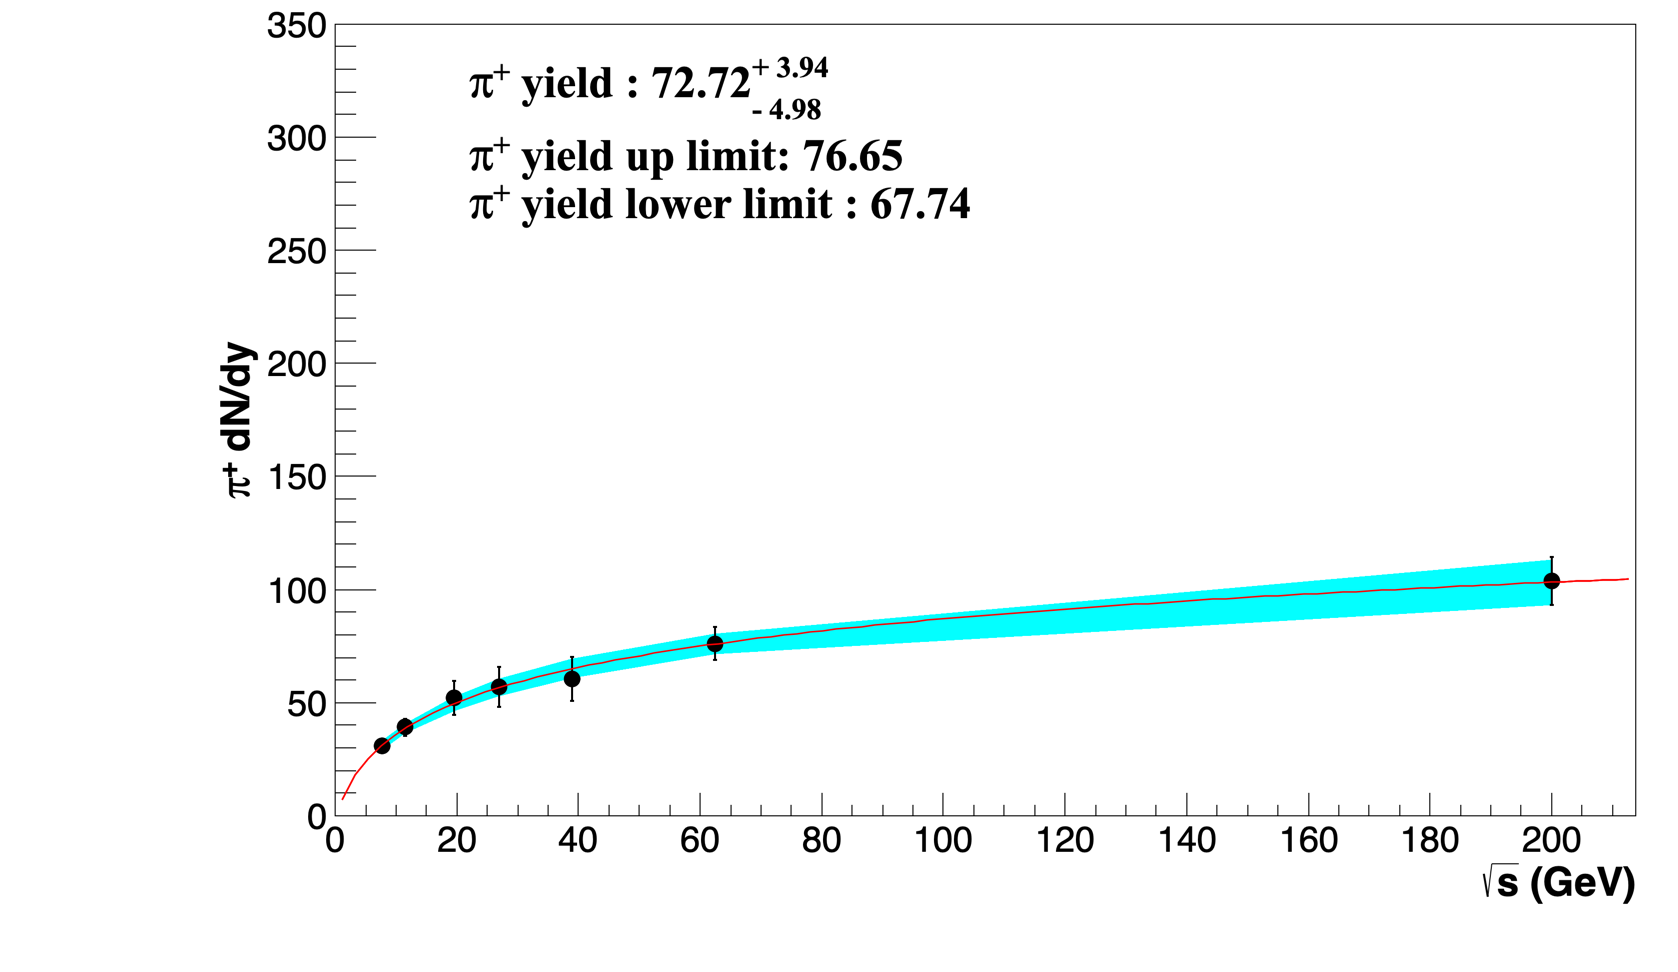
\includegraphics[width=\textwidth,clip]{figures/Chapter4/080_Plus_Yield.png}
        \caption{}
        \label{fig:pi_plus_yield}
    \end{subfigure}
    \hfill
    \begin{subfigure}[b]{0.45\textwidth}
        \centering
        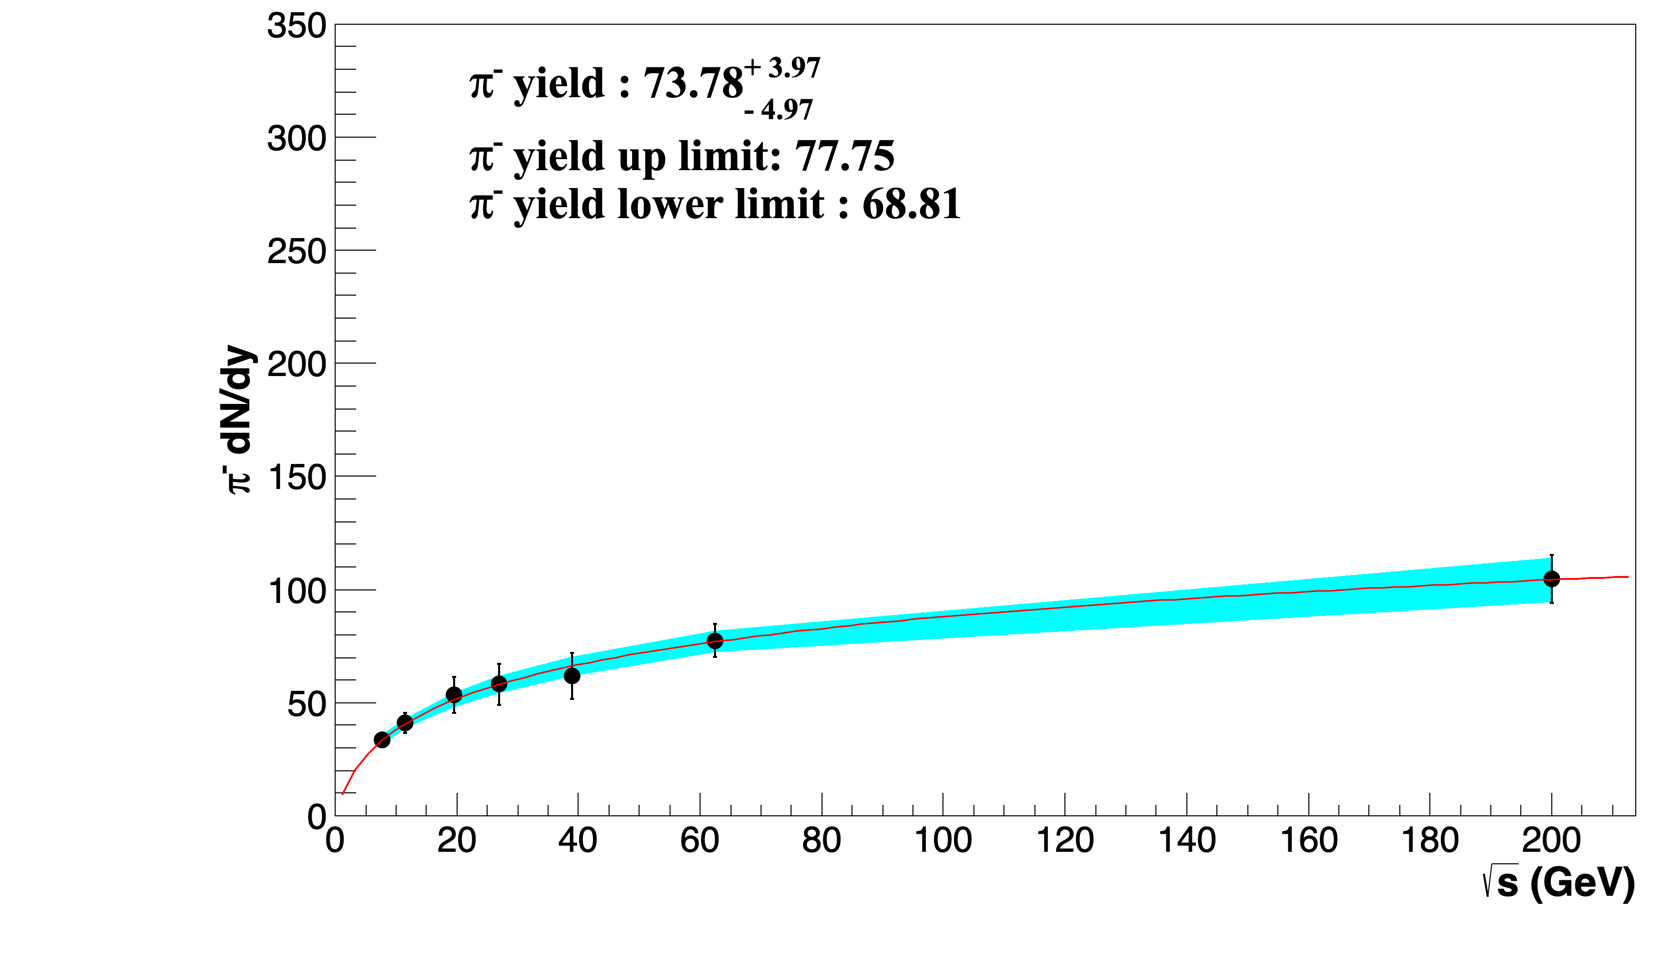
\includegraphics[width=\textwidth,clip]{figures/Chapter4/080_Minus_Yield.png}
        \caption{}
        \label{fig:pi_minus_yield}
    \end{subfigure}
    \caption[0-80\%中心度下$\pi^+$和$\pi^-$拟合的结果]{0-80\%中心度下$\pi^+$和$\pi^-$拟合的结果,左图为$\pi^+$的结果,右图为$\pi^-$的结果}
    \label{fig:pi_yield}
\end{figure}
\begin{table}[h!]
    \centering
    \caption{\sNN = 54.4 GeV 金-金对撞中不同中心度下$\pi^+$和$\pi^-$产额的值}
    \label{tab:pi_yield}
    \begin{tabularx}{0.8\textwidth} {
    | >{\centering\arraybackslash}X |>{\centering\arraybackslash}X |>{\centering\arraybackslash}X | }
        \hline
        Centrality & $\pi^+$ & $\pi^-$   \\
        \hline
        0-80\% & $72.72^{+3.94}_{-4.98}$  & $73.78^{+3.97}_{-4.97}$   \\
        \hline
        0-10\% & $203.16^{+7.60}_{-10.59}$  &  $205.87^{+7.64}_{-10.50}$  \\
        \hline
        10-40\% & $98.09^{4.06}_{5.48}$  &  $99.54^{+4.18}_{-5.55}$  \\
        \hline
        40-80\% & $21.15^{+1.21}_{-1.49}$  &  $21.49^{+1.17}_{-1.45}$  \\
        \hline
    \end{tabularx}
\end{table}

为了让最后的强子产额更加精确,在本分析当中对位于信噪比较高区间的$\omega$和$\phi$强子的产额最后是用模拟的分布去拟合真实数据抽取得到。当通过上文所述的模拟过程得到强子衰变模拟双电子谱之后,再用得到的模拟双电子谱的形状分布作为输入,对数据进行拟合。就可以得到一个额外的整体归一化因子,并用这个因子对$\omega$和$\phi$模拟谱进行归一化,使其可以更好地描述数据。在拟合的时候,整个用来拟合的强子衰变模拟的分布被分成了四部分,如式\ref{eq:float_meson}所示。其中$N_{total-\omega-\phi}$,$N_{\omega}$,$N_{\phi}$分别为总的强子衰变模拟去掉$\omega$以及$\phi$的分布、$\omega$的强子衰变模拟分布和$\phi$的强子衰变模拟分布 。$n_{broaden~\rho}$为broaden $\rho$模型中的$\rho$的分布。a、b、c、d为模拟各个分布的归一化系数。0-80\%中心度下的拟合结果如图\ref{fig:float_meson} 所示。不同中心度下的拟合参数的结果如表\ref{tab:float_meson}所示。在此拟合当中,只有$n_{\omega}$,$n_{\phi}$以及$n_{broaden~\rho}$的产额作为自由参数参与拟合,$n_{total-\omega-\phi}$被固定为1。

\begin{equation}
    \label{eq:float_meson}
    n_{fit} = a*n_{total-\omega-\phi}+b*n_{\omega}+c*n_{\phi}+d*n_{broaden~\rho}
\end{equation}

\begin{figure}[htb]
    \begin{center}
    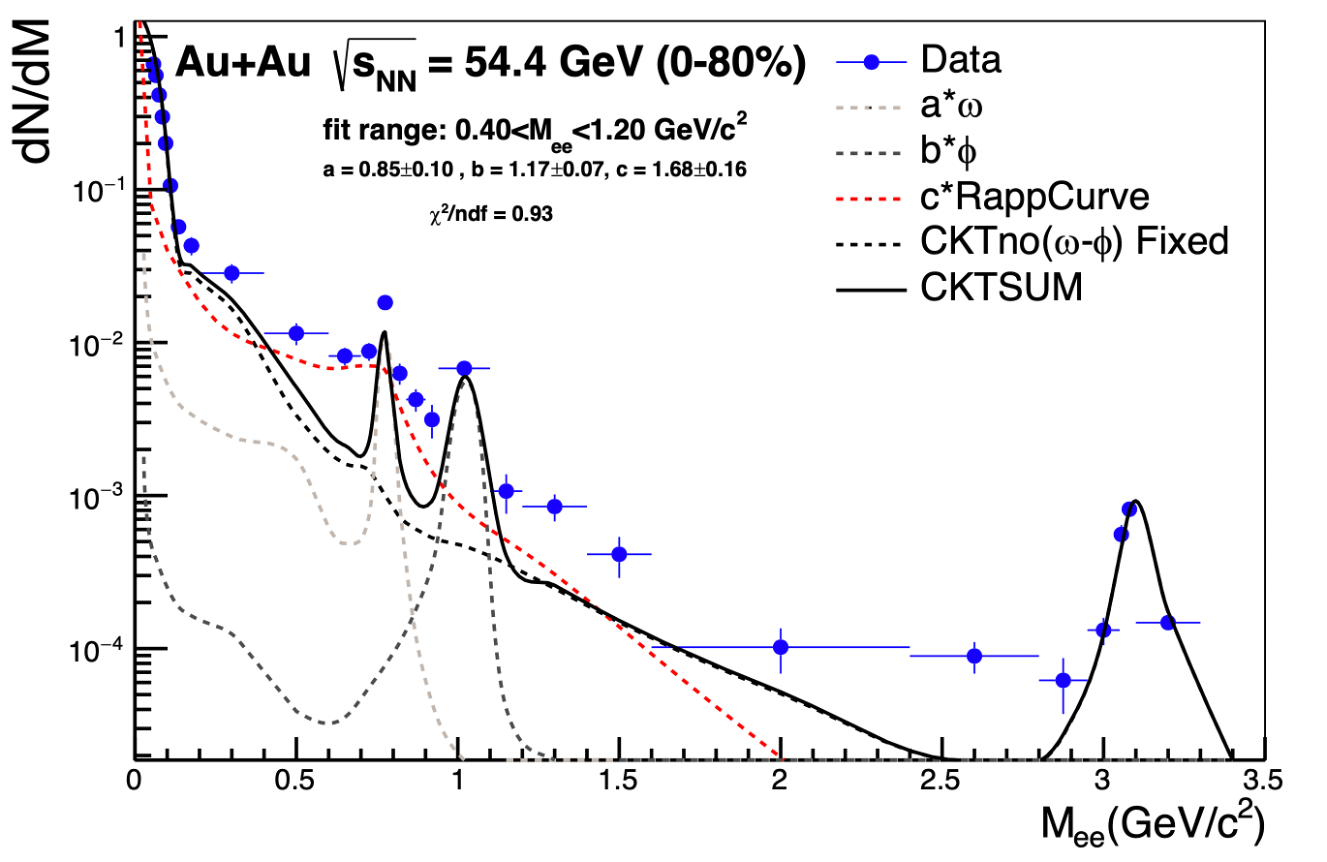
\includegraphics[width=0.75\textwidth,clip]{figures/Chapter4/float_meson.png}
    \end{center}
    \caption[强子衰变模拟对数据的拟合结果示意图]{\sNN = 54.4 GeV金-金对撞当中0-80\%中心度下强子衰变模拟对数据的拟合结果,其中蓝点为数据点,不同的拟合分量在图中用不同形式的线标出。各个分量的拟合参数已列在图中}
    \label{fig:float_meson}
\end{figure}

\begin{table}[h!]
    \centering
    \caption{54.4GeV金-金对撞中不同中心度下式\ref{eq:float_meson}中拟合参数的拟合结果}
    \label{tab:float_meson}
    \begin{tabularx}{0.8\textwidth} {
    | >{\centering\arraybackslash}X |>{\centering\arraybackslash}X |>{\centering\arraybackslash}X |>{\centering\arraybackslash}X |>{\centering\arraybackslash}X | }
        \hline
        Centrality & a & b & c & d   \\
        \hline
        0-80\%  & 1 & $0.85 \pm 0.10$ & $1.17 \pm 0.07$ & $1.68 \pm 0.16$ \\
        \hline
        0-10\%  & 1 & $0.90 \pm 0.20$ & $1.35 \pm 0.17$ & $1.42 \pm 0.27$ \\
        \hline
        10-40\% & 1 & $0.86 \pm 0.10$ & $1.14 \pm 0.08$ & $1.53 \pm 0.17$ \\
        \hline
        40-80\% & 1 & $1.05 \pm 0.09$ & $1.07 \pm 0.07$ & $2.58 \pm 0.20$ \\
        \hline
    \end{tabularx}
\end{table}


\subsection{重味夸克半轻子衰变}

在中等质量区间,来源于重味夸克半轻子衰变的双轻子对占了主要的部分。我们使用PYTHIA6作为模拟的产生子来得到模拟结果。由PYTHIA6产生的质子-质子对撞中的结果经过归一化和乘以$N_{bin}$后与介子模拟的结果加在一起后与最终的测量结果进行比较。在本小节中将对整个模拟过程进行详细介绍。因为在低能量下,相比于c夸克的截面b夸克的截面很小可以忽略不计,所以在本分析中仅对c夸克的贡献进行模拟。

对于PYTHIA6产生子,在本分析中基本沿用STAR的模拟设置,但对以下几个参数进行了调整:MSEL = 4(c trigger); PARP(91) = 1 $<k_T>$ = 1.0 GeV/c; PARP(61) = 1 (parton shower level tuning)
同时为了提高模拟的效率,对于产生的含c夸克的介子,在产生子当中将不含电子的衰变道关闭。

通过PYTHIA得到的来源于c夸克半轻子衰变的双电子分布经过式\ref{eq:Nor_c}归一化之后再与测量结果进行比较。其中$\sigma_{cc}$和$\sigma_{mb}$分别为金-金对撞中c夸克和最小无偏对撞的截面,$N_{bin}$为不同中心度下的二元碰撞数。BR为含c夸克介子到电子或者正电子的分支比。
\begin{equation}
    \label{eq:Nor_c}
    \frac{dN}{dM} = \frac{1}{N_{evt}} (\frac{dN}{dM})_{pp} \frac{\sigma_{cc}}{\sigma_{mb}} N_{bin} (BR_{c~\rightarrow e^+}) (BR_{c~\rightarrow e^-})
\end{equation}

同样由于 \sNN = 54.4 GeV 金-金对撞的数据中缺少对c夸克截面的测量,仍然需要通过拟合的方式来外推c夸克的截面。在本分析当中收集了STAR在其他能量下和其他实验的测量结果,通过拟合的方式来外推\sNN = 54.4 GeV下c夸克的截面。拟合结果如图\ref{fig:Charm_Xsection}所示。通过拟合得到的c夸克截面为${\rm 72.49 \mu b}$。$N_{bin}$通过STAR官方的中心度定义包RefMult给出,在不同中心度下的结果如表\ref{tab:Nbin}所示。
\begin{figure}[htb]
    \begin{center}
    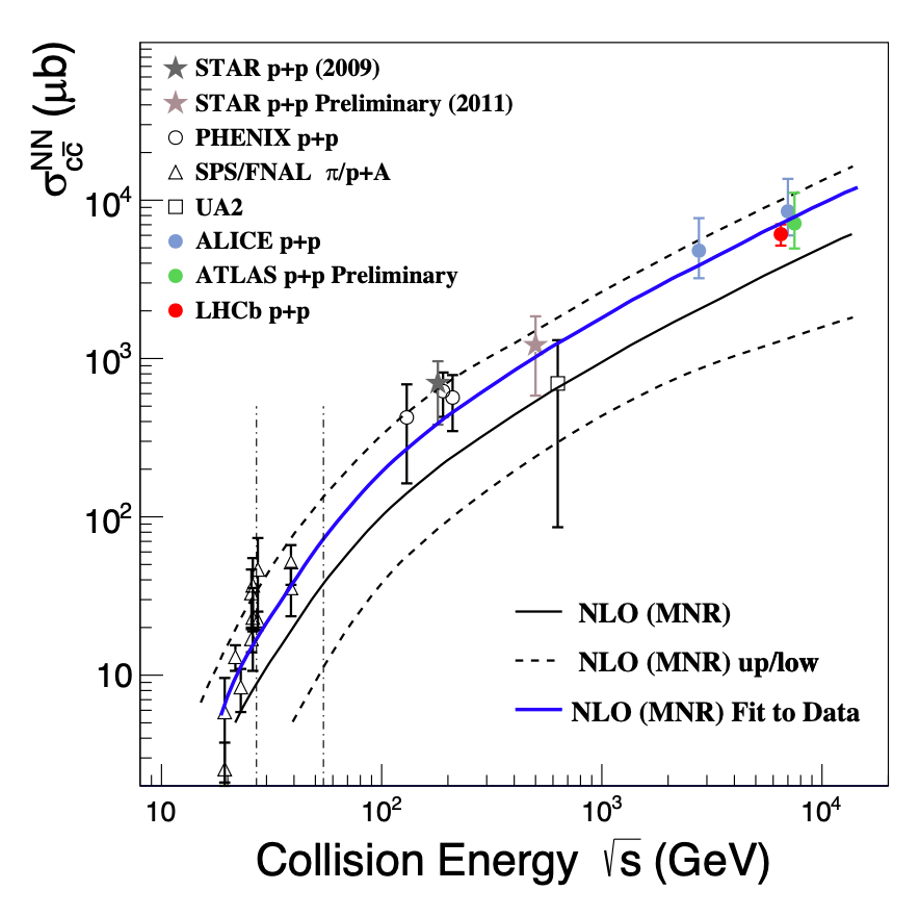
\includegraphics[width=0.8\textwidth,clip]{figures/Chapter4/CharmXsession.png}
    \end{center}
    \caption[c夸克截面拟合结果]{c夸克截面拟合结果,拟合曲线为NLO(MNR)理论计算曲线}
    \label{fig:Charm_Xsection}
\end{figure}
\begin{table}[h!]
    \centering
    \caption{\sNN = 54.4 GeV 金-金对撞中不同中心度下$N_{bin}$的值}
    \label{tab:Nbin}
    \begin{tabularx}{0.8\textwidth} {
    | >{\centering\arraybackslash}X  |>{\centering\arraybackslash}X | }
    \hline
    Centrality & $N_{bin}$ \\
    \hline
    0-80\% & 257.20 \\
    \hline
    0-10\% & 811.80 \\
    \hline
    10-40\% & 342.06 \\
    \hline
    40-80\% & 51.22 \\
    \hline
    \end{tabularx}
\end{table}

测量的初期在如何对c夸克的贡献进行归一化的时候遇到了问题,最开始产生的源自c夸克的双电子模拟谱和STAR BES-1的结果进行比较时发现两边的结果无法匹配,\sNN = 54.4 GeV的结果甚至低于\sNN = 39的c夸克的双轻子模拟谱的结果。后来经过和STAR之前\sNN = 200 GeV 金-金以及质子-质子对撞中的结果进行比较,发现在BES-1的分析和的\sNN = 200 GeV 金-金以及质子-质子对撞的分析当中在对源自c夸克的双电子模拟谱进行模拟的时候采用了两种不同的方法来决定$N_{evt}$的数目。这两种方法分别是:
\begin{itemize}
    \item[inclusive charm method] : $N_{evt}$为在进行模拟时至少有一个c或者 ${\rm \bar{c}}$夸克的事例数
    \item[2 c string method] : $N_{evt}$为在模拟时同时有一个c string 和 ${\rm \bar{c}}$ string的事例数 
\end{itemize}
inclusive charm method 被应用在了\sNN = 200 GeV 金-金以及质子-质子对撞的分析当中,而 2 c string method 被应用在了BES-1的分析当中。

对于双轻子测量来说,之所以要做$1/N_{mb}$的归一化是因为测量的是在一个最小无偏对撞中的双轻子的产额,所以在做模拟的归一化时,所用的总事例数$N_{evt}$应该满足式\ref{eq:N_decay}。这样选取$N_{evt}$就应该和我们计算$\sigma_{c\bar{c}}$时的方法相同。在测量$\sigma_{c\bar{c}}$时是通过测量open charm的产额确定其在中间快度区域的截面后再去反推在全空间的截面。所以$N_{evt}$应该是在模拟当中可以发现open charm的事例数。而在进一步的检查当中发现在PYTHIA6的模拟当中如果事例里面没有2 charm string仍然可以在末态的粒子当中找到来源于open charm的电子对。所以\sNN = 200 GeV测量中使用的确定$N_{evt}$更加合理。为了对这种方法进行验证,在用这种方法模拟产生\sNN = 200 GeV质子-质子对撞当中的重味夸克半轻子衰变的双轻子谱后和STAR之前发表的\sNN = 200 GeV质子-质子对撞中的双轻子谱进行比较,发现可以很好的描述之前的测量数据。所以inclusive charm method被确定为最后的$N_{evt}$数目的选择方法。
\begin{equation}
    \label{eq:N_decay}
    N_{mb} = N_{evt}*\frac{\sigma_{mb}}{\sigma_{c\bar{c}}}
\end{equation}

\subsection{Drell-Yan 过程}
当对撞的质心能量降低的时候,Drell-Yan过程产生的双电子产额和由璨夸克产生的双电子产额处在同一个数量级。所以在模拟过程中不能忽略来自于Drell-Yan过程的双电子。在进行归一化时所用到的归一化公式和璨夸克模拟的模拟时所用到的类似。Drell-Yan过程的模拟也面临着和璨夸克模拟时类似的问题,缺少截面$\sigma_{DY}$的测量。

在STAR之前的双电子谱测量当中,\sNN = 19.6 GeV的测量能量与本分析接近且在其强子衰变模拟中包含了Drell-Yan过程,其中$\sigma_{DY}$为 9.88 nb\cite{STAR:2015zal}。而在Pythia当中,默认的\sNN = 19.6 GeV下的$\sigma_{DY}$为13.44 nb。这两个值之间的比值被用作修正因子来修正\sNN = 54.4 GeV Pythia默认的$\sigma_{DY}$的值来外推得到\sNN = 54.4 GeV中的$\sigma_{DY}$。外推公式和结果如式\ref{eq:DY}所示。
\begin{equation}
    \label{eq:DY}
    \begin{split}
        \rm{ \sigma_{DY} = \sigma_{DY}^{Pythia}*\frac{\sigma_{DY}^{19.6~GeV~papaer}}{\sigma_{DY}^{19.6~GeV~Pythia}} = 19.25 nb } \\
        \rm{  \sigma_{DY}^{54.4~GeV~Pythia} = 26.19 nb }
    \end{split}
\end{equation}
\subsection{ \textbf{$p_T$ smearing} }

为了让模拟的结果可以更好的反应探测器的分辨率带来的影响,在进行强子衰变模拟的时候需要对末态粒子的横动量相对于模拟的值添加一个小的增量。这个增量可以为正值也可以是负值。这个添加增量的过程被称作$p_T$ smearing。

在STAR官方的模拟(embedding)当中,已可以在一定程度上反应探测器对径迹动量的影响。但因为时间投影室当中可以影响到最后横动量测量结果的因素多且复杂,以及STAR的高亮度的测量环境本身也会对横动量的测量带来影响,这就使得embedding中的探测器的分辨率相比于真实情况更加的精确。即在相同动量下同一个粒子(如$J/\psi$)的谱的宽度会变得比测量结果更窄。这就需要调整$p_T$ smearing的参数使得模拟结果可以更好的描述数据。

首先需要确定描述得到探测器的分辨率的方法。在embedding的数据当中,可以得到$\delta_{p_T}/p_T ~v.s.~p_T$的二维分布。将数据分成多个不同的$p_T$区间,各个区间内在 $\delta_{p_T}/p_T$的峰值附近进行高斯拟合,得到的高斯拟合的宽度便可以确定在每个$p_T$区间内的探测器的分辨,如图\ref{fig:Pt_res}所示。
探测器的分辨$\sigma_{p_T}/p_T$随$p_T$变化的曲线,如图\ref{fig:pT_res_embd}所示。其中拟合曲线为式\ref{eq:pT_res}。当得到a的值之后,接下来要做的就是对在一定变化范围内对a的值进行扫描,从而对描述探测器分辨的方程进行标定,从而确定可以最好地描述数据的a的值。
\begin{figure}[htb]
    \centering
    \begin{subfigure}[b]{0.45\textwidth}
        \centering
        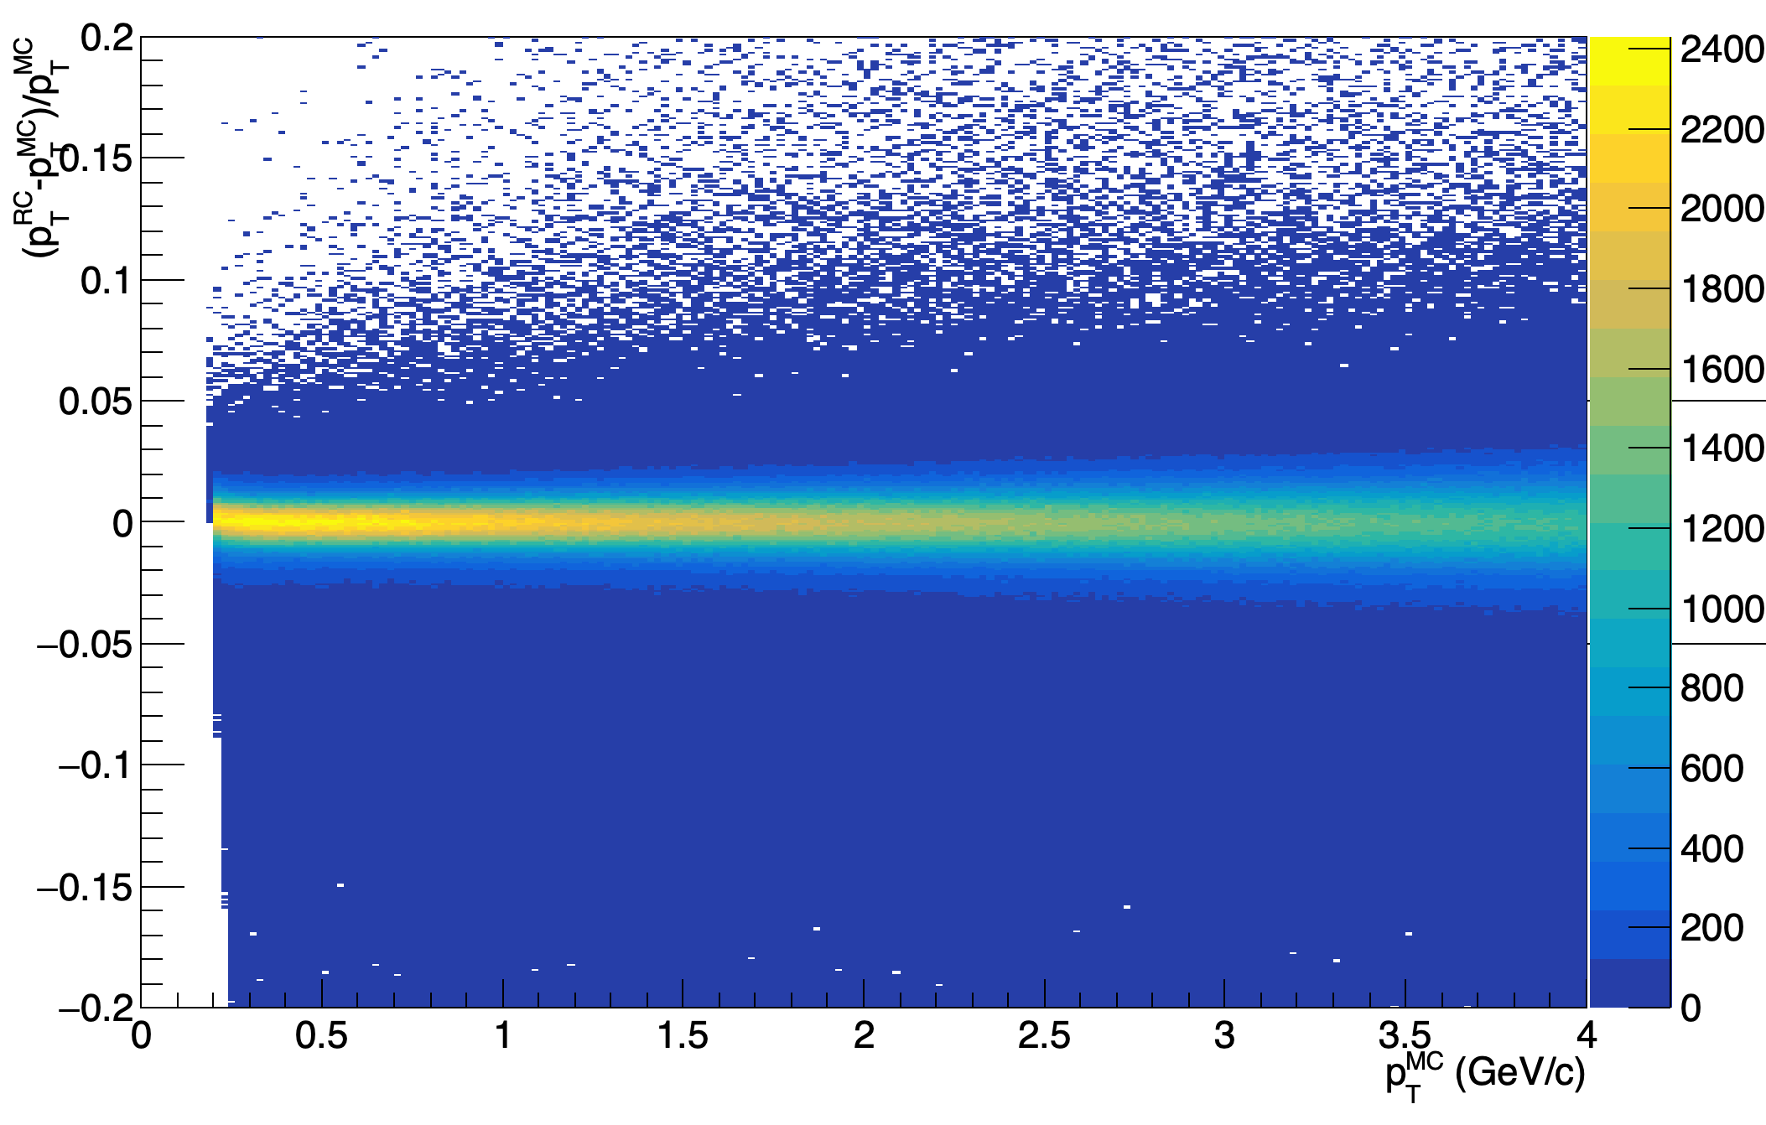
\includegraphics[width=\textwidth,clip]{figures/Chapter4/Pt_res_2D.png}
        \caption{}
        \label{fig:Pt_res_2D}
    \end{subfigure}
    \hfill
    \begin{subfigure}[b]{0.45\textwidth}
        \centering
        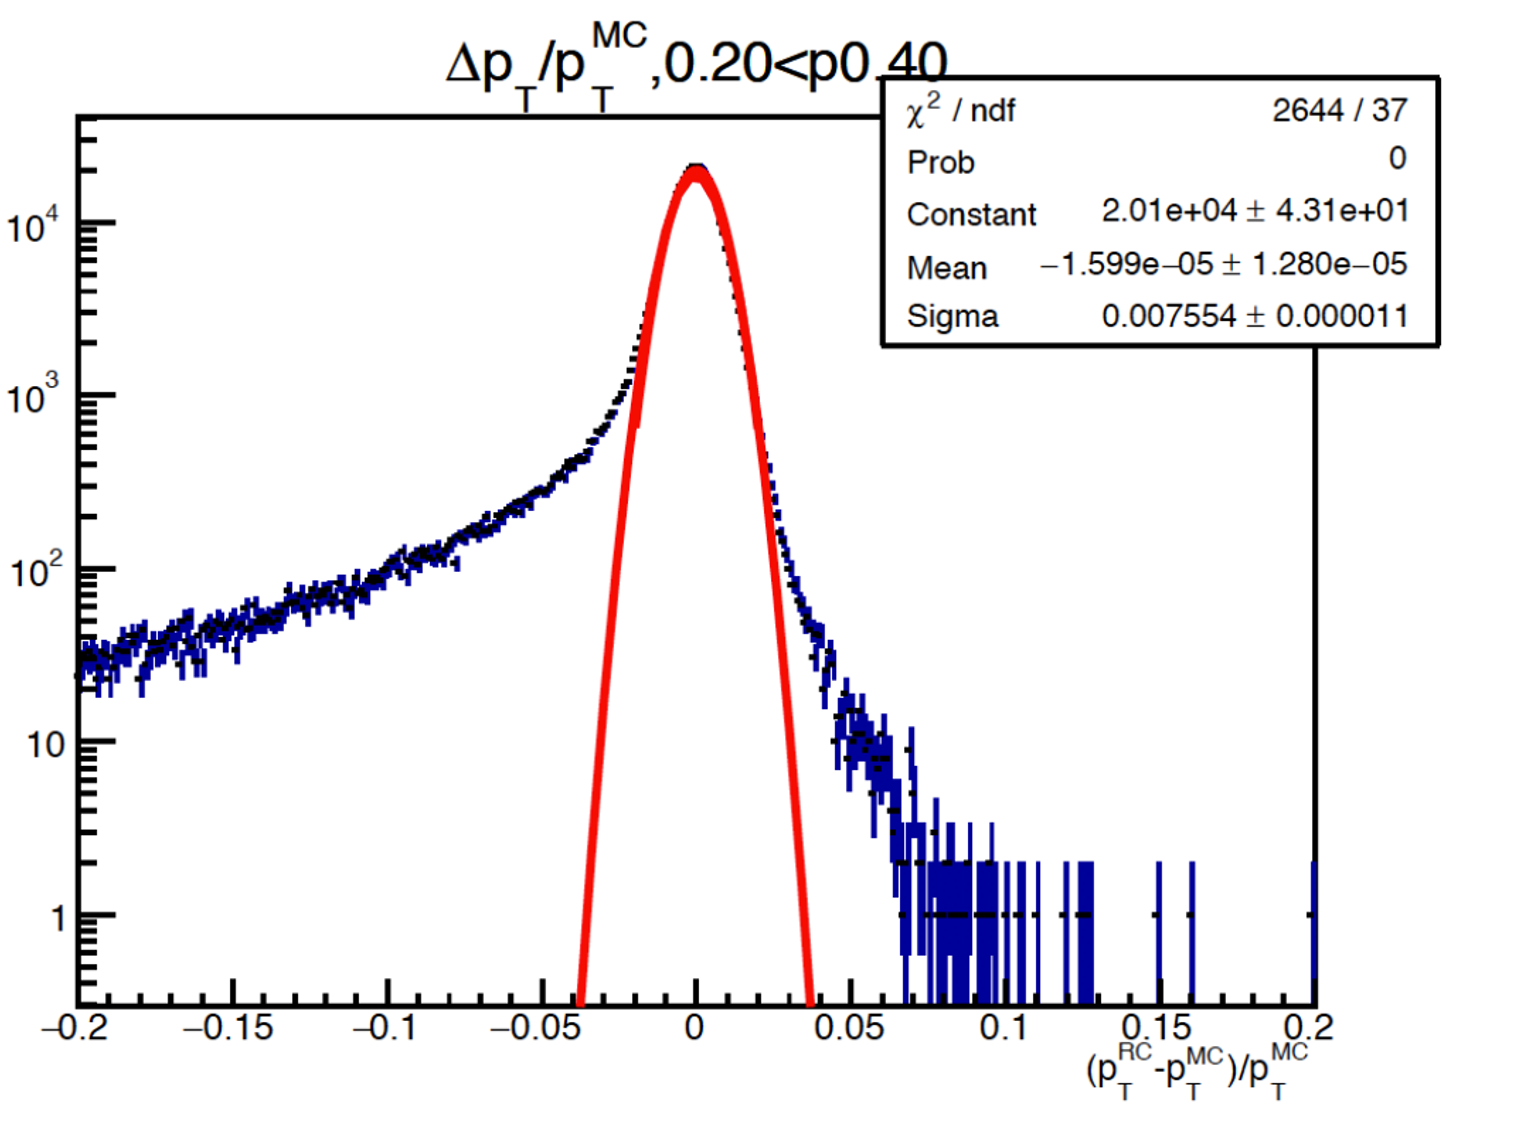
\includegraphics[width=\textwidth,clip]{figures/Chapter4/Pt_res_fit.png}
        \caption{}
        \label{fig:Pt_res_fit}
    \end{subfigure}
    \caption[0-80\%中心度下embedding 中的$\delta_{p_T}/p_T$分布示意图]{0-80\%中心度下embedding 中的$\delta_{p_T}/p_T$分布示意图,左图为$ \sigma_{p_T}/p_T~v.s.~p_T$的二维分布。右图为 $\rm{0.2 < p_T < 0.4~GeV/c}$ 区间内的拟合结果,拟合曲线为高斯函数。 }
    \label{fig:Pt_res}
\end{figure}
\begin{equation}
    \label{eq:pT_res}
    \delta_{p_T} = \sqrt{a^2 p_T^2 + b^2}
\end{equation}

\begin{figure}[htb]
    \begin{center}
    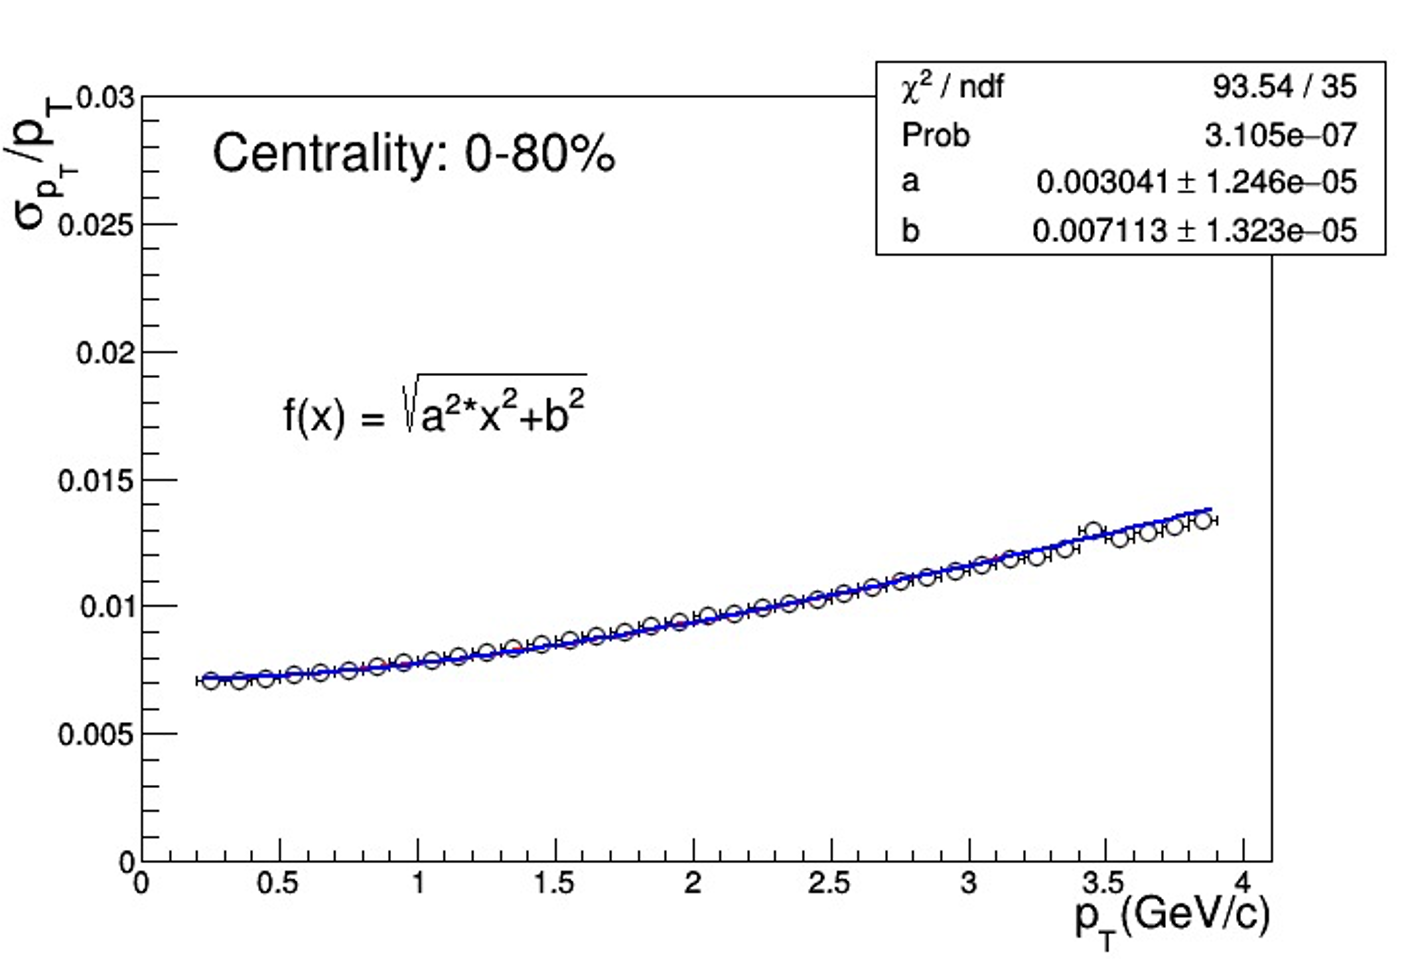
\includegraphics[width=0.8\textwidth,clip]{figures/Chapter4/pT_res_embd.png}
    \end{center}
    \caption[横动量分辨率随横动量变化示意图]{0-80\%中心度下横动量分辨率随横动量变化示意图,并通过拟合得到$\sigma_{p_T}/p_T$随$p_T$变化的曲线,拟合方程在图中标出。}
    \label{fig:pT_res_embd}
\end{figure}

因为$\rm{J/\psi}$有着信噪比高的优势,所以在本分析当中$\rm{J/\psi}$的信号被选取用来作为标定的参考信号。以0-80\%中心度为例,首先在0.001-0.021的范围内每隔0.0001取一个不同的a的值。这些不同的a的值分别作为$p_T$ smearing输入的参数产生$\rm{J/\psi}$的模拟结果。再用这些不同的模拟结果去拟合数据中的$\rm{J/\psi}$分布。使拟合的$\chi^2$最小的a的值就是可以最好地描述数据的a的值,在相同中心度下不同的物理过程模拟中均使用这个值作为$p_T$ smearing参数。a值扫描结果如图\ref{fig:Chi2_TuneA}所示。在不同中心度下的a的值见表\ref{tab:a}。
\begin{figure}[htb]
    \begin{center}
    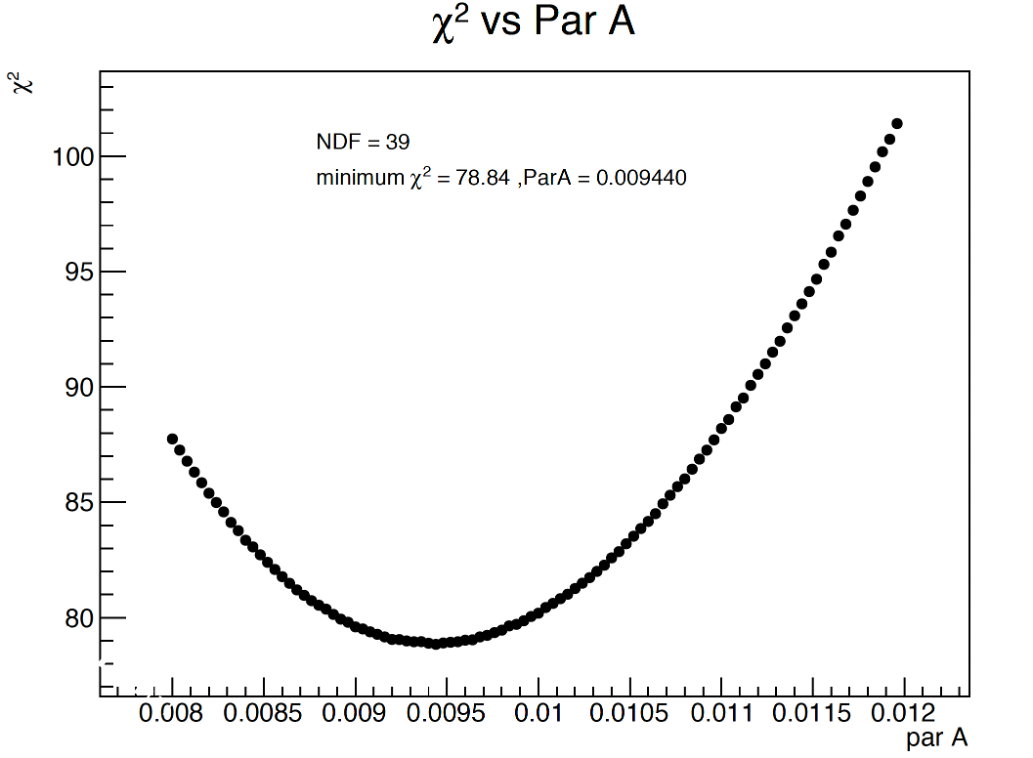
\includegraphics[width=0.8\textwidth,clip]{figures/Chapter4/Chi2_TuneA.png}
    \end{center}
    \caption[不同参数a时模拟样本拟合数据的$\chi^2$分布]{寻找最佳参数a时不同a下$\chi^2$的值}
    \label{fig:Chi2_TuneA}
\end{figure}
\begin{table}[h!]
    \centering
    \caption{\sNN = 54.4 GeV 金-金对撞中不同中心度下a的值}
    \label{tab:a}
    \begin{tabularx}{0.8\textwidth} {
    | >{\centering\arraybackslash}X  |>{\centering\arraybackslash}X | }
    \hline
    Centrality & a \\
    \hline
    0-80\% & 0.006450 \\
    \hline
    0-10\% & 0.005600 \\
    \hline
    10-40\% & 0.007700 \\
    \hline
    40-80\% & 0.008250 \\
    \hline
    \end{tabularx}
\end{table}